\section{Implementation}

\subsection{Web Technologies}
\label{sec:web_technologies}

As we saw above, I implemented my prototype as a web application. The criteria for picking an implementation platform was that of accessibility to users and speed of development. Using that criteria I decided to make my prototype a web application as its only entry barrier to users is that of a modern web browser. I took the Prov-O-Vis~\cite{Hoekstra2014} system as inspiration as it was the most accesible of the availble provenance visualisers and this is partially because it is available online. Web applications are a field that I have experience with and can quickly develop in. 

There are a few pitfalls to this approach that can be addressed through alternative implementations. Because my application is primarily a prototype for illustrating effective exploration features, the issue of scale is not one that is addressed. If a web application was used for enterprise size provenance files the application may run out of resources; further testing and alternative approaches may be required.

An alternative to a web application would be to write the prototye in an OS independent language such as Java or Python; this would allow wide accessibility and more fine grained control of machine resources. However if an OS level language was chosen issues could later occur in presenting provenance on mobile devices and a mobile version of the interface may need to be written. Alternatively if an OS dependant language such as Apple's swift of Microsoft's C\# was used features and code would have to be replicated for the different OS languages (assuming that OS independent accessibility is an important criteria).

The standard technology for data visualisation in a browser is the D3.js\footnote{D3: Data Driven Documents \url{https://d3js.org/}} JavaScript library. However as mentioned earlier, I used Cytoscape.js to implement my interface because it is specifically focused on graph theory and has a graph functions built in (such as distance algorithms). 

\subsection{Client Side Processing}
\label{sec:client_side_processing}

When a provenance file is selected ProvOwl loads the file and renders it all locally. When first outlining features of the application I wanted it to be primarily stand alone. This means that even though it can run from a web server, you could just as easily run it locally on your computer with minimal effort as all computations are done client side.

However server side computation may be a useful feature for the future, a server with higher computational power and resources may be able to find and analyze interesting details about a file. A simple approach to accomplish this would to have the file uploaded to the server, analytics run on the provenance and then results loaded back to the client. For larger provenance files this could be extended to only load sections required for analysis reducing the bandwidth required. The client could render the provenance locally whilst results where computed and then rendered onto the already drawn graph. This would allow the user to begin exploring the graph with minimal delay while extra information is calculated server side.

\subsection{Node Clustering}

Creating a clustering functino in Cytoscape.js required some time and effort because it currently doesn't have a clustering feature, so I was required to write one from scratch. The goal of this function was to have grouping and ungrouping nodes been undestructive: if a series of nodes are grouped and then ungrouped the resulting graph should be isomorphic to the original.

\begin{figure}[h]
  \centering
  \begin{subfigure}[t]{0.5\textwidth}
    \includegraphics[width=\textwidth]{ungrouped}
    \caption{A provenance graph showing information about a report given on twitter data.}
  \end{subfigure}
  ~
  \begin{subfigure}[t]{0.5\textwidth}
    \includegraphics[width=\textwidth]{grouped}
	\caption{The nodes \texttt{Tweets} and \texttt{X-tweets-[1-3]} have been clustered into the composite node \texttt{uwJIJ}}
  \end{subfigure}
  \caption{A provenance that has had a subset of its nodes clustered. In an early version of the prototype composite nodes were given random alphanumeric names as seen on the right.}
\end{figure}

Nodes removed from Cytoscape.js can be `restored' into their original position, unfortunately any edged associated with a removed node are permanently destroyed. It is necessary then to store the edges as a data field in the composite node so that when restoring nodes, edges can also be recreated. 

The pseudocode below creates a new cluster. It creates a new node and stores the selected nodes and their edges as properties of it. Then new edges are created from surrounding nodes to the composite node. Finally the selected nodes are ``removed'' so that they are no longer visible.

\begin{figure}[h]
  \centering
  \begin{lstlisting}
 // Create composite node 
 Create new CompositeNode 
 CompositeNode.originalEdges = All edges in neighbourhood of selected nodes // save edges
 CompositeNode.originalNodes = All nodes that where grouped // save nodes

 // Create new edges connected to the composite node
 for each edge in neighbourhood {
  if (edge IS NOT internal to group)  {
    Create new Edge({from: externalNode, to:compositeNode})
  }
 }

 // Remove original nodes
 Remove selected nodes
 \end{lstlisting}
 \caption{Pseudocode: Creaing a composite node}
\end{figure}

However the above code only works in a limited scenario: ungrouping nodes in the opposite order of creation. For example if you created composite nodes $A$, $B$, $C$ (chronologically and all with neighbouring edges) you would have to ungroup them in the following order: $C$, $B$, $A$. If you where to for example ungroup node $A$ first, when ungrouping $C$ it would try to restore edges to the now non-existenat $A$ compsosite node, there's an example of this in Figure~\ref{fig:clustring-without-groupmanager}. In order to fix this I created a class called group manager to monitor nodes in clusters.

The Group Manager class is the primary way of keeping track of nodes that are hidden inside composite nodes. It contains a tree data structure that references all the groups as well as their child nodes/groups. When ungrouping nodes this class is called and the parent group of the child node requested, then a new temporary edge is created to the composite node and the original edge stored in a \textit{hanging edges} object until it can be restored. Every time a group is created or destroyed the \textit{hanging edges} object is queried to see if any originl edges can be recreated, as seen in Figure~\ref{fig:clustring-with-groupmanager}.

\begin{figure}[h]

  \begin{subfigure}[t]{0.5\textwidth}
    \centering
    \begin{tikzpicture}
      \node[main node] (A1) {A1};
      \node[main node] (A2) [right of=A1] {A2};
      \node[main node] (B1) [below of=A1] {B1};
      \node[main node] (B2) [below of=A2] {B2};
      \path (A1) edge node[left] {used} (B1);
      \path (A2) edge node[left] {used} (B2);
    \end{tikzpicture}
    \caption{Nodes $A1$ and $B1$ are linked, nodes $A2$ and $B2$ are linked.}
  \end{subfigure}
  ~
  \begin{subfigure}[t]{0.5\textwidth}
    \centering
    \begin{tikzpicture}
      \node[main node, group] (CA) {CA};
      \node[main node] (B1) [below left of=CA] {B1};
      \node[main node] (B2) [below right of=CA] {B2};
      \path (CA) edge node[left] {used} (B1);
      \path (CA) edge node[right] {used} (B2);
    \end{tikzpicture}
    \caption{Group nodes $A1$ and $A2$ into composite node $CA$. Stored inside the composite node is the original edges from $A1\rightarrow B1$ and $A2\rightarrow B2$.}
  \end{subfigure}
  \begin{subfigure}[t]{0.5\textwidth}
    \centering
    \begin{tikzpicture}
      \node[main node, group] (CA) {CA};
      \node[main node, group] (CB) [below of=CA] {CB};
      \path (CA) edge node[right] {used} (CB);
    \end{tikzpicture}
    \caption{Group nodes $B1$ and $B2$ insto composite nodes $CB$. Stored inside the composite node $CB$ is the edges from $CA\rightarrow B1$ and $CA\rightarrow B2$.}
  \end{subfigure}
  ~
  \begin{subfigure}[t]{0.5\textwidth}
    \centering
    \begin{tikzpicture}
      \node[main node, group] (CB) {CB};
      \node[main node] (A1) [above left of=CB] {A1};
      \node[main node] (A2) [above right of=CB] {A2};
    \end{tikzpicture}
    \caption{Ungroup $CA$. It will try to create adges between $A1\rightarrow B1$ and $A2\rightarrow B2$, because $B1$ and $B2$ are currently in a group, the new edges will fail and not be rendered.}
  \end{subfigure}
  \begin{subfigure}[t]{0.5\textwidth}
    \centering
    \begin{tikzpicture}
      \node[main node] (A1) {A1};
      \node[main node] (A2) [right of=A1] {A2};
      \node[main node] (B1) [below of=A1] {B1};
      \node[main node] (B2) [below of=A2] {B2};
    \end{tikzpicture}
    \caption{Ungroup $CB$. Edges between $CA\rightarrow B1$ and $CA\rightarrow B2$ will try to be restored but because there's no $CA$ in the graph these will fail.}
  \end{subfigure}
  \caption{An example of issues that occur when trying to ungroup nodes in the incorrect order without the \textit{Group Manager}. As seen in the final step, the original edges connecting the nodes are lost.}
\end{figure}

\begin{figure}[h]

  \begin{subfigure}[t]{0.5\textwidth}
    \centering
    \renewcommand\thesubfigure{A1}
    \begin{tikzpicture}
      \node[main node] (A1) {A1};
      \node[main node] (A2) [right of=A1] {A2};
      \node[main node] (B1) [below = 1cm of A1] {B1};
      \node[main node] (B2) [below = 1cm of A2] {B2};
      \path (A1) edge node[left] {used} (B1);
      \path (A2) edge node[left] {used} (B2);
    \end{tikzpicture}
    \caption{Nodes $A1$ and $B1$ are linked, nodes $A2$ and $B2$ are linked.}
  \end{subfigure}
  ~
  \begin{subfigure}[t]{0.5\textwidth}
    \renewcommand\thesubfigure{A2}
    \centering
    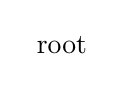
\begin{tikzpicture}
      \node[] (root) {root};
    \end{tikzpicture}
    \caption{The GMTree (Group Manager Tree) is currently empty and Hangingedges = [].}
  \end{subfigure}
  \begin{subfigure}[t]{0.5\textwidth}
    \centering
    \renewcommand\thesubfigure{B1}
    \begin{tikzpicture}
      \node[main node, group] (CA) {CA};
      \node[main node] (B1) [below left of=CA] {B1};
      \node[main node] (B2) [below right of=CA] {B2};
      \path (CA) edge node[left] {used} (B1);
      \path (CA) edge node[right] {used} (B2);
    \end{tikzpicture}
    \caption{Group nodes $A1$ and $A2$ into composite node $CA$. Stored inside the composite node is the original edges from $A1\rightarrow B1$ and $A2\rightarrow B2$.}
  \end{subfigure}
  ~
  \begin{subfigure}[t]{0.5\textwidth}
    \centering
    \renewcommand\thesubfigure{B2}
    \begin{tikzpicture}
      \node[] (root) {root};
      \node[below = 1cm of root] (CA) {CA};
      \node[below right = 1cm of CA] (A1) {A1};
      \node[below left = 1cm of CA] (A2) {A2};
      \path (root) edge (CA);
      \path (CA) edge (A1);
      \path (CA) edge (A2);
    \end{tikzpicture}
    \caption{The GMTree holds information about $CA$, $A1$ and $A2$. Hangingedges = [].}
  \end{subfigure}

  \begin{subfigure}[t]{0.5\textwidth}
    \renewcommand\thesubfigure{C1}
    \centering
    \begin{tikzpicture}
      \node[main node, group] (CA) {CA};
      \node[main node, group] (CB) [below of=CA] {CB};
      \path (CA) edge node[right] {used} (CB);
    \end{tikzpicture}
    \caption{Group nodes $B1$ and $B2$ insto composite nodes $CB$. Stored inside the composite node $CB$ is the edges from $CA\rightarrow B1$ and $CA\rightarrow B2$.}
  \end{subfigure}
  ~
  \begin{subfigure}[t]{0.5\textwidth}
    \centering
    \renewcommand\thesubfigure{C2}
    \begin{tikzpicture}
      \node[] (root) {root};
      \node[below right = 1cm of root] (CA) {CA};
      \node[below right = 0.5cm of CA] (A1) {A1};
      \node[below left = 0.5cm of CA] (A2) {A2};

      \node[below left = 1cm of root] (CB) {CB};
      \node[below right = 0.5cm of CB] (B1) {B1};
      \node[below left = 0.5cm of CB] (B2) {B2};
      \path (root) edge (CA);
      \path (CA) edge (A1);
      \path (CA) edge (A2);
      \path (root) edge (CB);
      \path (CB) edge (B1);
      \path (CB) edge (B2);
    \end{tikzpicture}
    \caption{The GMTree holds information about all nodes. Hangingedges = [].}
  \end{subfigure}

  \begin{subfigure}[t]{0.5\textwidth}
    \centering
    \renewcommand\thesubfigure{D1}
    \begin{tikzpicture}
      \node[main node, group] (CB) {CB};
      \node[main node] (A1) [above left of=CB] {A1};
      \node[main node] (A2) [above right of=CB] {A2};
      \path (A1) edge node[left] {used} (CB);
      \path (A2) edge node[right] {used} (CB);
    \end{tikzpicture}
    \caption{CA is ungrouped and removed from the group manager tree. The original edges $A1\rightarrow B1$ and $A2\rightarrow B2$ can not be restored because B1 and B2 aren not in the graph, these edges are stored in the hanging edges object. New edges are created by finding the prent node using the group manager.}
	\label{fig:clustring-without-groupmanager}
  \end{subfigure}
  ~
  \begin{subfigure}[t]{0.5\textwidth}
    \centering
    \renewcommand\thesubfigure{D2}
    \begin{tikzpicture}
      \node[] (root) {root};
      \node[below = 1cm of root] (CB) {CB};
      \node[below right = 0.5cm of CB] (B1) {B1};
      \node[below left = 0.5cm of CB] (B2) {B2};
      \path (root) edge (CB);
      \path (CB) edge (B1);
      \path (CB) edge (B2);
    \end{tikzpicture}
    \caption{The GMTree holds information about $B$ nodes. $A$ nodes have been remove because they've been ungrouped. Hangingedges = [$A1\rightarrow B1$, $A2\rightarrow B2$].}
  \end{subfigure}

  \begin{subfigure}[t]{0.5\textwidth}
    \centering
    \renewcommand\thesubfigure{E1}
    \begin{tikzpicture}
      \node[main node] (A1) {A1};
      \node[main node] (A2) [right of = A1] {A2};
      \node[main node] (B1) [below = 1cm of A1] {B1};
      \node[main node] (B2) [below = 1cm of A2] {B2};
      \path (A1) edge node[left] {used} (B1);
      \path (A2) edge node[left] {used} (B2);
    \end{tikzpicture}
    \caption{CB is ungrouped and removed from the group manager tree. An attempt to restore hanging edges is made and both $A1\rightarrow B1$ and $A2\rightarrow B2$ are restored.}
  \end{subfigure}
  ~
  \begin{subfigure}[t]{0.5\textwidth}
    \centering
    \renewcommand\thesubfigure{E2}
    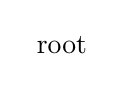
\begin{tikzpicture}
      \node[] (root) {root};
    \end{tikzpicture}
    \caption{The GMTree is empty because there's no groups. Hangingedges = [] because the previously stored edges have been restored.}
  \end{subfigure}
  \caption{The same example as in Figure~\ref{fig:clustring-without-groupmanager} except this time using the group manager and hanging edges. The group manager stores a tree to track groups and internal nodes as seen on the right hand side. Hanging edges stores a list of edges that have not been restored yet because one or more connected nodes were missing.}
	\label{fig:clustring-with-groupmanager}
\end{figure}
